\section{Auswertung}

\subsection{Messung der geometrischen Abmessungen}

\subsection{Widerstandsmessung}
Für die Proben Zink und Kupfer wurde jeweils die Spannung in Abhängigkeit vom Strom gemessen. Die Messwerte befinden sich
%in den Tabellen \ref{tab: uri_zink} und \ref{tab: uri_kupfer}.

\begin{minipage}{\textwidth}
 \begin{tabular}{S S } 
 \toprule  
 {$I$ in $\si{\ampere}$} & {$U$ in $\si{\volt}$}   \\ 
\midrule  
 0.0 & 0.0  \\ 
0.8 & 6.6  \\ 
1.6 & 12.5  \\ 
2.4 & 18.6  \\ 
3.2 & 24.7  \\ 
4.0 & 30.8  \\ 
4.8 & 37.0  \\ 
5.6 & 43.3  \\ 
6.4 & 49.6  \\ 
7.2 & 55.6  \\ 
8.0 & 63.4  \\ 
\bottomrule 
 \end{tabular} 
 \caption{Zinkprobe: Messung der Spannung in Abhängigkeit vom Strom } 
 \label{tab: uri_zink}
\hfill
\begin{table} 
\centering 
\caption{Kupferprobe: Messung der Spannung in Abhängigkeit vom Strom } 
\label{tab: uri_kupfer} 
\begin{tabular}{S S } 
\toprule  
{$I$ in $\si{\ampere}$} & {$U$ in $\si{\volt}$}   \\ 
\midrule  
 0.0  & 0.0\\ 
1.0  & 7.8\\ 
2.0  & 15.5\\ 
3.0  & 23.2\\ 
4.0  & 31.0\\ 
5.0  & 38.5\\ 
6.0  & 46.3\\ 
7.0  & 53.8\\ 
8.0  & 61.5\\ 
9.0  & 68.8\\ 
10.0  & 76.5\\ 
\bottomrule 
\end{tabular} 
\end{table}
\end{minipage}

Die Auftragung der Messwerte sowie die Regressionsgeraden sind in den Abbildungen \ref{fig: uri_zink} und \ref{fig: uri_kupfer} illustriert.
Als Regressionsparamter für die Steigungen, die den Widerständen entsprechen, ergeben sich die Werte:
\begin{equation}
  R_{Cu} = (7.64 \pm 0.02)\si{\milli \ohm} \quad \quad R_{Zn} = (7.80 \pm 0.06)\si{\milli \ohm}
\end{equation}
\FloatBarrier
\begin{figure}
  \centering
  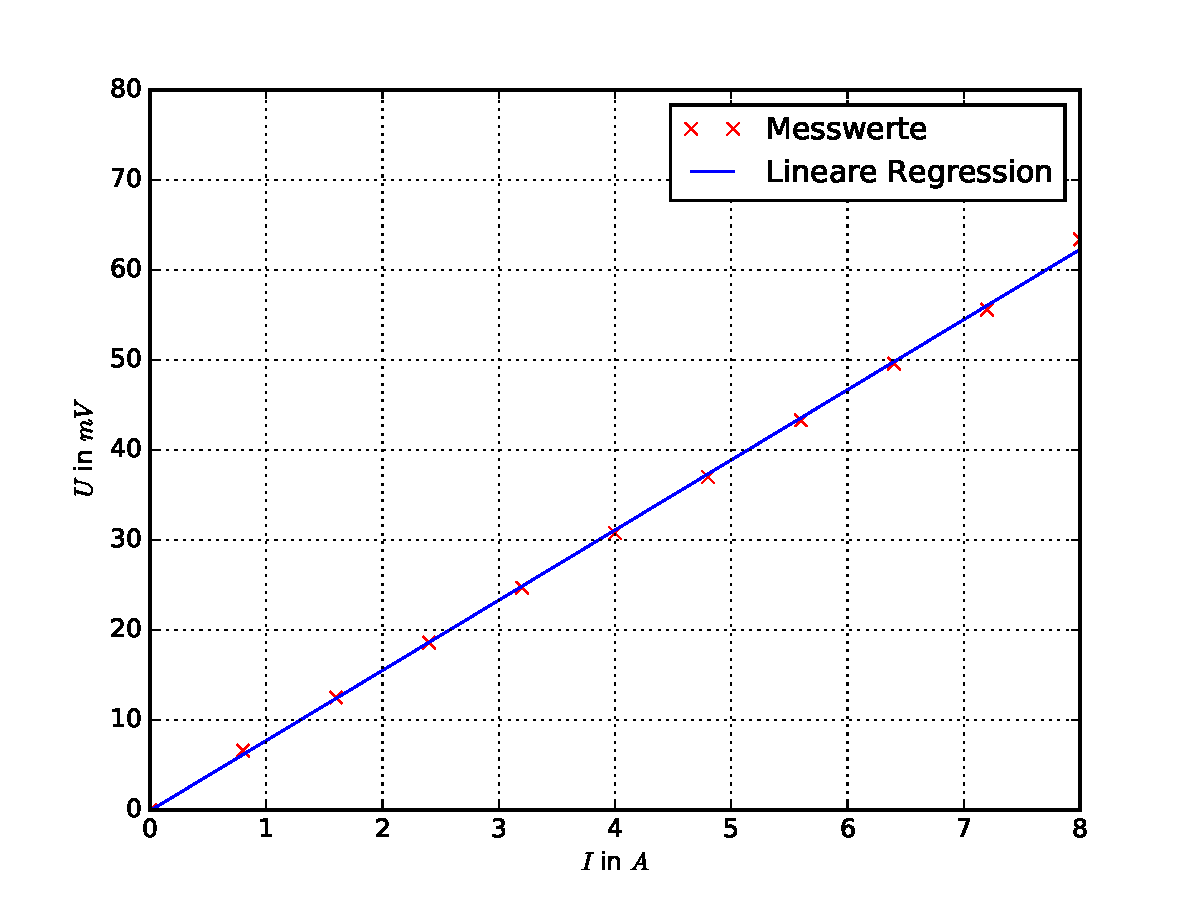
\includegraphics[width=\textwidth]{pics/uri_zink.pdf}
  \caption{Zinkprobe Verlauf der Spannung in Abhängigkeit vom Strom}
  \label{fig: uri_zink}
\end{figure}
\begin{figure}
  \centering
  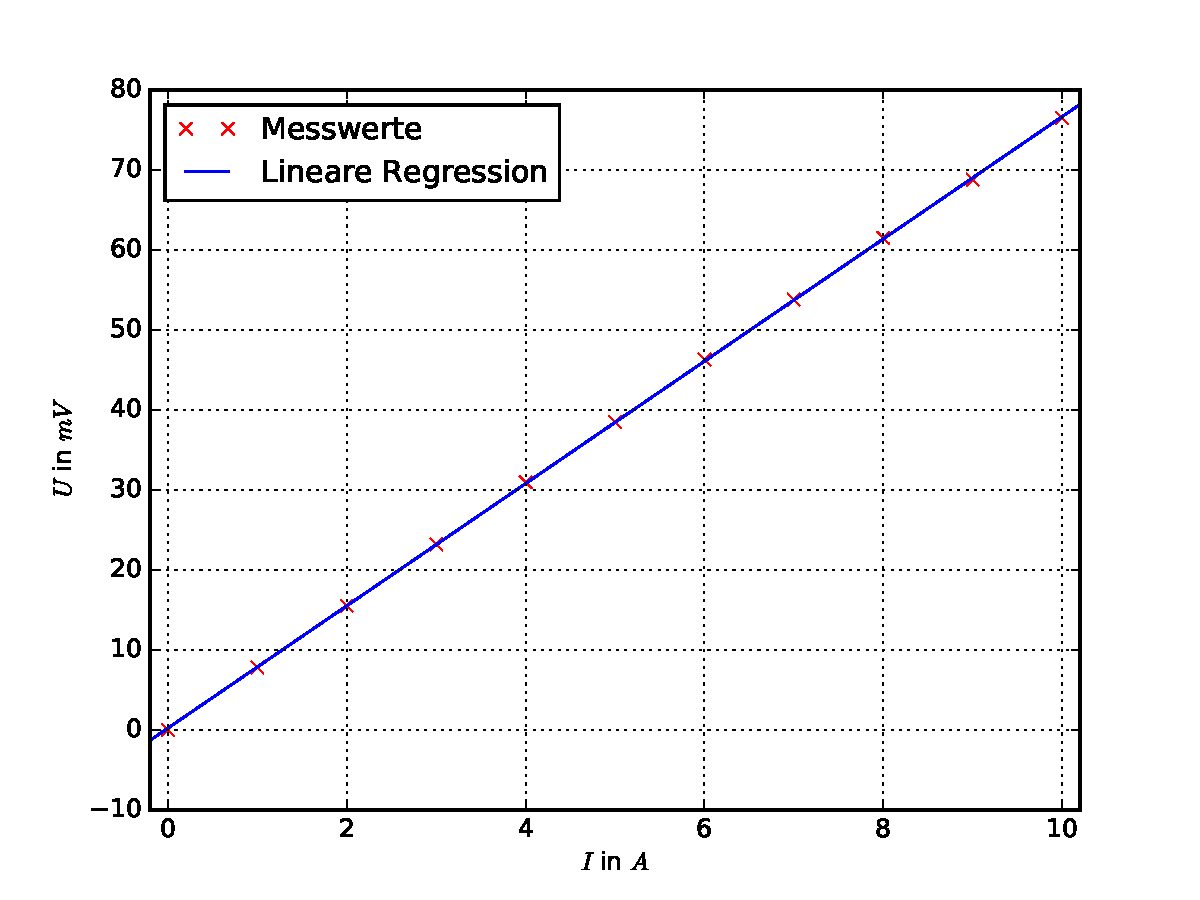
\includegraphics[width=\textwidth]{pics/uri_kupfer.pdf}
  \caption{Kupferprobe Verlauf der Spannung in Abhängigkeit vom Strom}
  \label{fig: uri_kupfer}
\end{figure}



\subsection{Magnetfeldmessung}
Die Werte aus der Messung des Magnetfeldes in Abhängigkeit vom Spulenstrom sind in Tabelle \ref{tab: hysterese} einzusehen.
Hierbei entsprechen $B_{wachsend}$ bzw. $B_{fallend}$ den gemessenen magnetischen Flussdichten bei wachsendem
bzw. fallendem Spulenstrom.
Die graphische Darstellung (Abbildung \ref{fig: hysterese}) zeigt, dass die Hysterese-Effekte vernachlässigbar sind. Für
spätere Berechnungen soll der Zusammenhang zwischen dem ansteigendem Spulenstrom $I$ und dem dadurch entstehenden
Magnetfeld mittels linearer Regression an eine Gerade approximiert werden. Für die Steigung $m$ und den $y\,$-Achsenabschnitt $b$ ergeben sich:
\begin{equation}
  m = (-219.4 \pm 4.3) \si{\milli\tesla \per \ampere} \quad b =  (1.1 \pm 12.8) \si{\milli\tesla}
  \label{eq: hysterese}
\end{equation}
Die Regressiongerade ist ebenfalls in Abbildung \ref{fig: hystrese} dargestellt. Die Koeffizienten \eqref{eq: hysterese} werden im Folgenden
als Fehlerunbehaftet angenommen.
\begin{table} 
 \centering 
 \begin{tabular}{S S S } 
 \toprule  
{$I_q$ in $\si{\ampere}$} & {$B_{wachsend}$ in $\si{\milli \tesla}$}  &  {$B_{fallend}$ in $\si{\milli \tesla}$}  \\ 
\midrule  
 0.0  & -5.6  & -28.2\\ 
0.5  & -69.0  & -144.4\\ 
1.0  & -208.9  & -269.8\\ 
1.5  & -330.1  & -392.4\\ 
2.0  & -453.5  & -517.6\\ 
2.5  & -573.2  & -624.8\\ 
3.0  & -671.2  & -729.6\\ 
3.5  & -784.9  & -831.1\\ 
4.0  & -887.0  & -918.9\\ 
4.5  & -977.0  & -1002.0\\ 
5.0  & -1060.0  & -1060.0\\ 
\bottomrule 
 \end{tabular} 
 \caption{Messung des magnetischen Feldes bei fallendem und steigendem Strom} 
 \label{tab: hysterese} 
  \end{table}
\begin{figure}
  \centering
  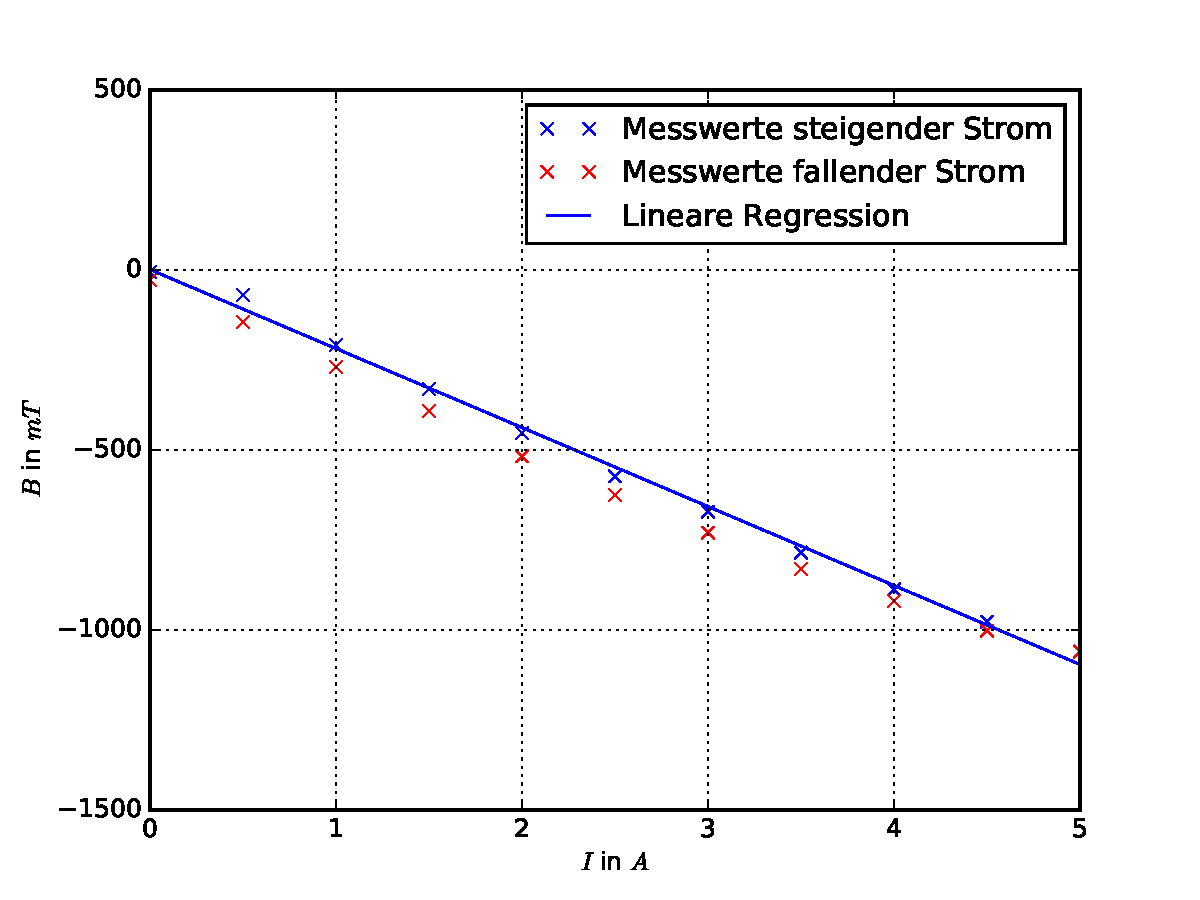
\includegraphics[width=\textwidth]{pics/hysterese.pdf}
  \caption{Verlauf der magnetischen Flussdichte in Abhängigkeit vom Spulenstrom}
  \label{fig: hysterese}
\end{figure}




\subsection{Hallspannung bei konstantem Magnetfeld}
Zur Messung der Hallspannung bei konstantem Magnetfeld wurde für beide Proben der Spulenstrom auf $3\si{\ampere}$ eingestellt. Die
Messwerte für $U_{ges+}$ und $U_{ges-}$ sowie die gemäß \eqref{eq:} berechneten Hallsapnnungen bei variablem Querstrom sind in den
Tabellen \ref{tab: } und \ref{tab: } aufgelistet. Eine weitere Regressionsrechnung ermöglicht mittels Gleichung \eqref{eq: } eine
erste Bestimmung der jeweiligen Teilchenzahl $n$ pro Volumen. Für die Beträge der jeweiligen Steigungen ergeben sich:
\begin{equation}
  m_{Cu} = (1.23 \pm 0.02)\si{\milli \volt \per \ampere}  \quad m_{Zn} = (1.63 \pm 0.24)\si{\milli \volt \per \ampere}
\end{equation}
Die Plots befinden sich in den Abbildungen \ref{fig: uh_konstB_kupfer} und \ref{fig: uh_konstB_zink}.
Damit ergeben sich die Werte für die Teilchenzahlen pro Volumen zu:
\begin{equation}
  n_{Cu,1} = (1.85 \pm 0.03)\cdot 10^{29}\,\si{ \meter^{-3}} \quad n_{Zn,1} = (1.68\pm 0.24)\cdot 10^{25}\,\si{ \meter^{-3}}
\end{equation}
\begin{table} 
 \centering 
 \begin{tabular}{S S S S } 
 \toprule  
 {$I$ in $\si{\ampere}$} & {$U_{ges-}$ in $\si{\milli \volt}$}  &  {$U_{ges+}$ in $\si{\milli \volt}$} & {$U_{H}$ in $\si{\milli \volt}$} \\ 
\midrule  
 0.0 & -0.336 & -0.338 & -0.001 \\ 
1.0 & -0.338 & -0.337 & 0.001 \\ 
2.0 & -0.340 & -0.336 & 0.002 \\ 
3.0 & -0.341 & -0.335 & 0.003 \\ 
4.0 & -0.343 & -0.335 & 0.004 \\ 
5.0 & -0.345 & -0.334 & 0.005 \\ 
6.0 & -0.346 & -0.333 & 0.006 \\ 
7.0 & -0.348 & -0.332 & 0.008 \\ 
8.0 & -0.350 & -0.331 & 0.009 \\ 
9.0 & -0.351 & -0.331 & 0.010 \\ 
10.0 & -0.353 & -0.330 & 0.011 \\ 
\bottomrule 
 \end{tabular} 
 \caption{Hallspannung Kupfer bei konstantem Magnetfeld} 
 \label{tab: hall_kupfer_konstB} 
  \end{table}
\begin{table} 
 \centering 
 \begin{tabular}{S S S S } 
 \toprule  
 {{$I$ in $\si{\ampere$}} & {{$U_{ges-}$ in $\si{\milli \volt$}}  &  {{$U_{ges+}$ in $\si{\milli \volt$}} & {{$U_{H}$ in $\si{\milli \volt$}} \\ 
\midrule  
 0.0 & -0.339 & -0.339 & 0.000 \\ 
1.0 & -0.426 & -0.429 & -0.002 \\ 
2.0 & -0.517 & -0.520 & -0.002 \\ 
3.0 & -0.603 & -0.610 & -0.004 \\ 
4.0 & -0.692 & -0.699 & -0.004 \\ 
5.0 & -0.777 & -0.795 & -0.009 \\ 
6.0 & -0.870 & -0.885 & -0.008 \\ 
7.0 & -0.959 & -0.975 & -0.008 \\ 
8.0 & -1.045 & -1.064 & -0.010 \\ 
9.0 & -1.128 & -1.151 & -0.012 \\ 
10.0 & -1.220 & -1.261 & -0.020 \\ 
\bottomrule 
 \end{tabular} 
 \caption{Hallspannung Zink bei konstantem Magnetfeld} 
 \label{tab: hall_zink_konstB} 
  \end{table}
\begin{figure}
  \centering
  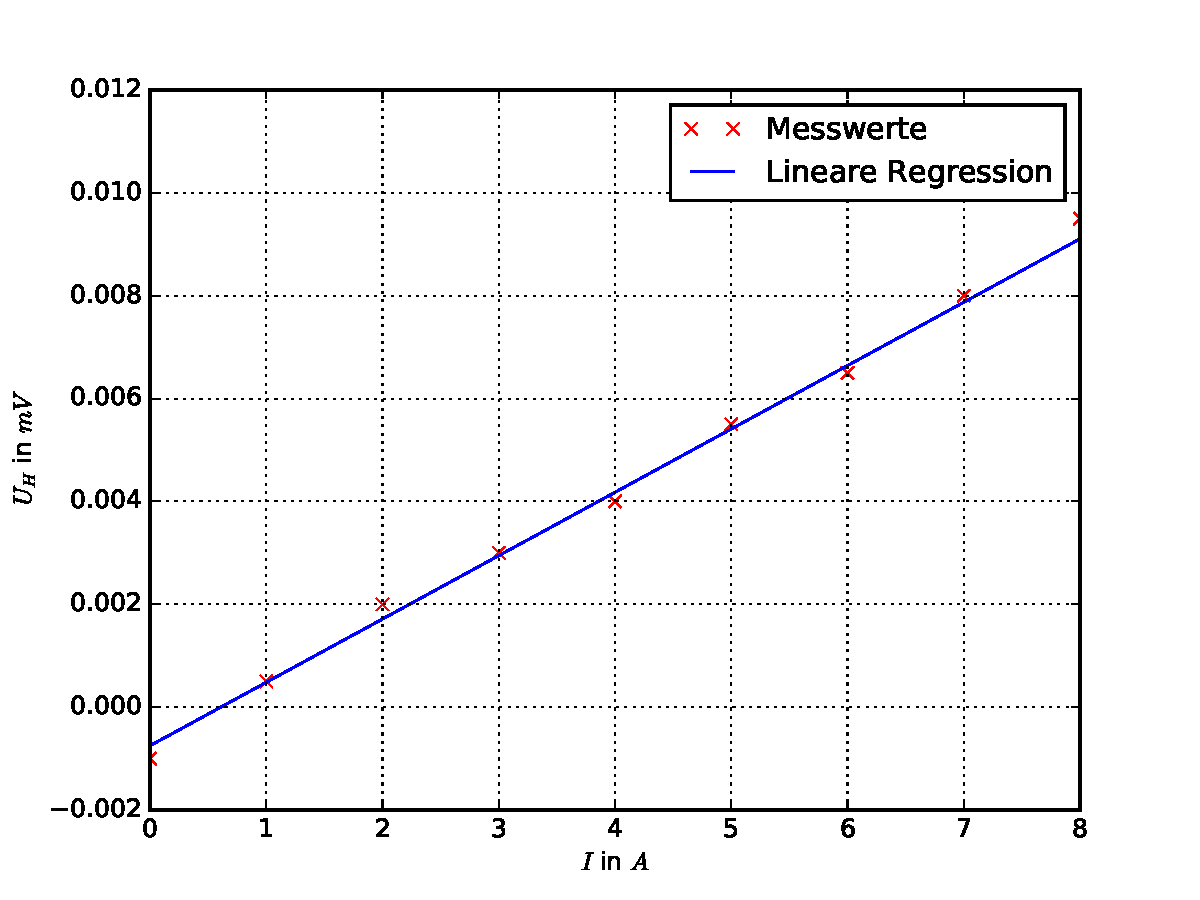
\includegraphics[width=\textwidth]{pics/u_h_kupfer_konstB.pdf}
  \caption{Kupferprobe, Verlauf der Hallspannung in Abhängigkeit vom Querstrom}
  \label{fig: uh_konstB_kupfer}
\end{figure}
\begin{figure}
  \centering
  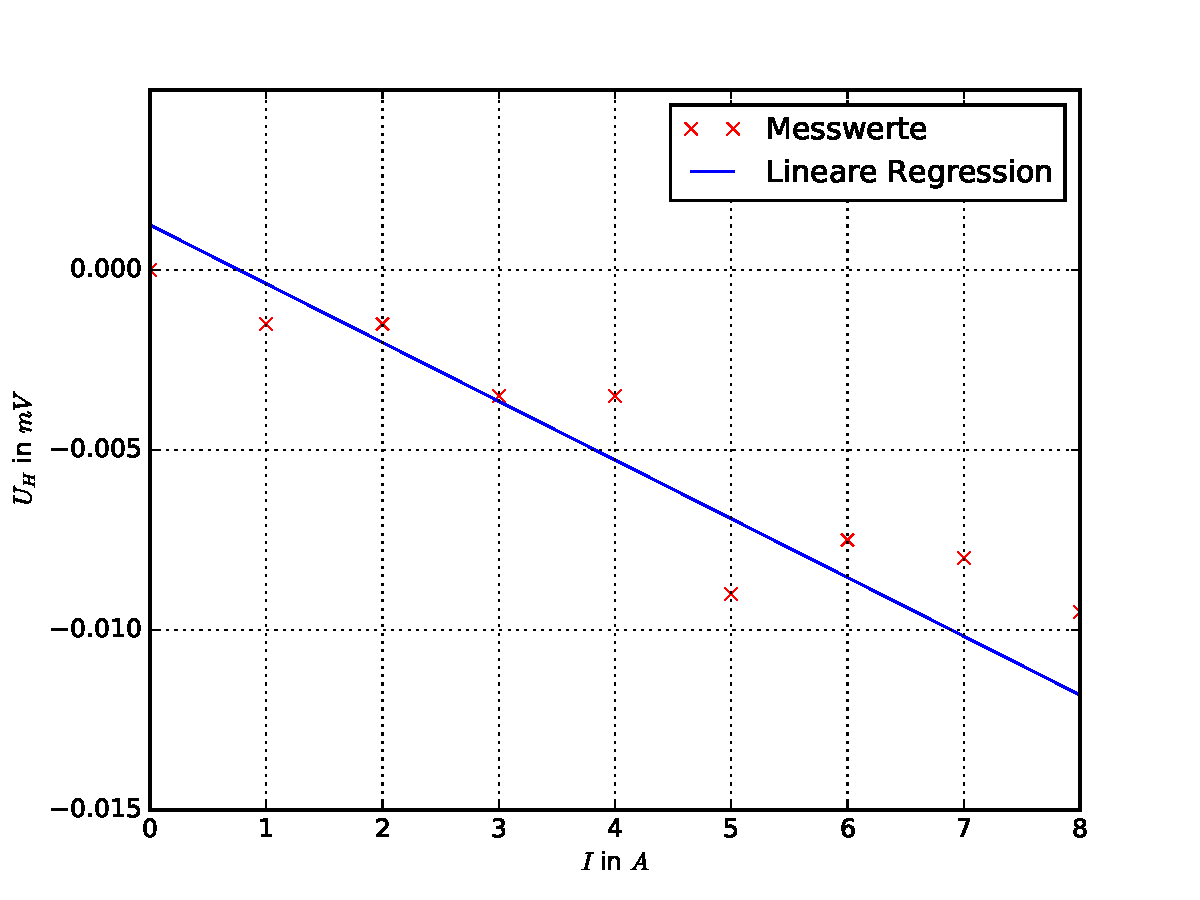
\includegraphics[width=\textwidth]{pics/u_h_zink_konstB.pdf}
  \caption{Zinkprobe, Verlauf der Hallspannung in Abhängigkeit vom Querstrom}
  \label{fig: uh_konstB_zink}
\end{figure}


\subsection{Hallspannung bei konstantem Querstrom}
